%%% template.tex
%%%
%%% This LaTeX source document can be used as the basis for your technical
%%% paper or abstract. Intentionally stripped of annotation, the parameters
%%% and commands should be adjusted for your particular paper - title, 
%%% author, article DOI, etc.
%%% The accompanying ``template.annotated.tex'' provides copious annotation
%%% for the commands and parameters found in the source document. (The code
%%% is identical in ``template.tex'' and ``template.annotated.tex.'')

\documentclass[conference]{acmsiggraph}

\TOGonlineid{45678}
\TOGvolume{0}
\TOGnumber{0}
\TOGarticleDOI{1111111.2222222}
\TOGprojectURL{}
\TOGvideoURL{}
\TOGdataURL{}
\TOGcodeURL{}

\title{A Hybrid Framework for Heterogeneous Crowd Simulation}

\author{Paper ID 116 Author One \\
		\thanks {anonymous@anonymous.edu} \\ Anonymous Univeristy
		\and
		Author Two \\
		\thanks {anonymous@anonymous.edu} \\ Anonymous Univeristy
		\and
		More Authors \\
		\thanks {anonymous@anonymous.edu} \\ Anonymous Univeristy
		\and}
\pdfauthor{}

\keywords{crowd simulation, hybrid algorithm, heterogeneous crowd, personal trait}

\begin{document}

%% \teaser{
%%   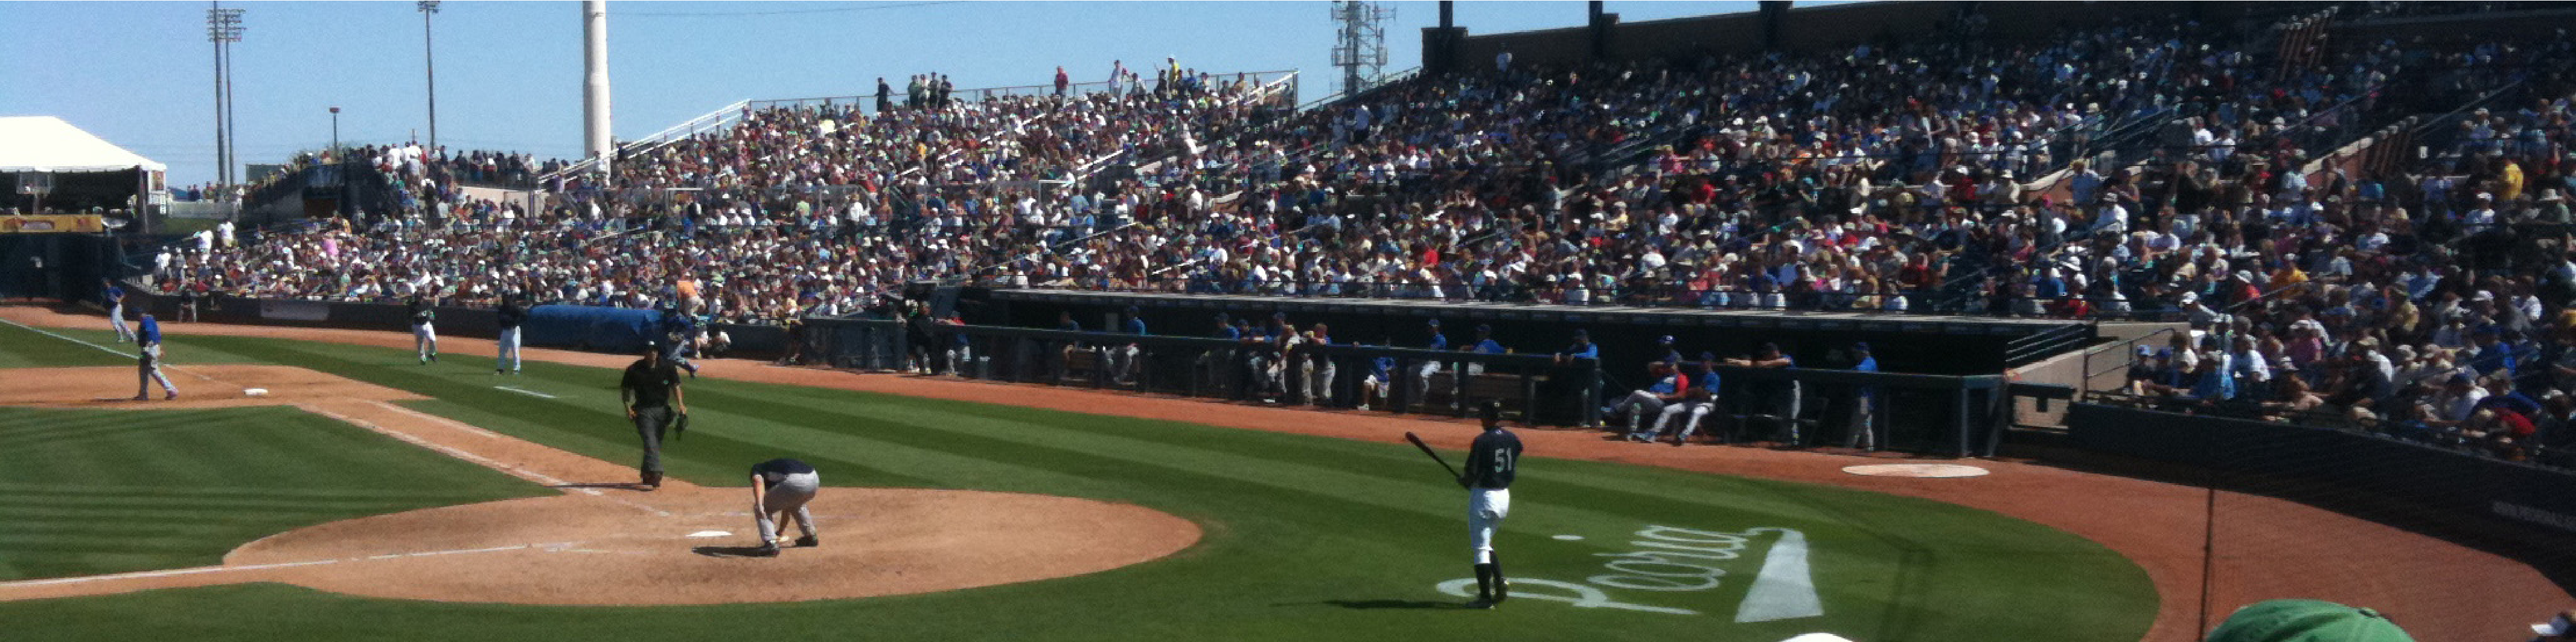
\includegraphics[height=1.5in]{images/sampleteaser}
%%   \caption{Spring Training 2009, Peoria, AZ.}
%% }

\maketitle

\begin{abstract}
The behavior of large human crowds is very complicated and subtle, because both physical factors (e.g., crowd density, agent velocity, agent position) and mental factors (e.g., personal traits) could have effect on local collision strategies. We present a novel hybrid framework to simulate heterogeneous crowds with various densities. In our approach, we define three types of interactions, agent-agent, agent-crowd, and intra-crowd, and integrate personal traits into all three of the interactions. We develop a Graph-Cut-based continuous crowd method to optimize the movement of agents in dense regions. We also introduce and give a solution to the avoid-or-join behavior when individual agents encounter dense crowds in their way. Finally, we demonstrate that we can get significant behavioral differences with different personality and density settings in simulations with our hybrid framework.

\end{abstract}

\begin{CRcatlist}
  \CRcat{I.3.7}{Computer Graphics}{Three-Dimensional Graphics and Realism}{Animation}
  \CRcat{I.2.11}{Artificial Intelligence}{Distributed Artificial Intelligence}{Multiagent systems}
\end{CRcatlist}

\keywordlist

%% Use this only if you're preparing a technical paper to be published in the 
%% ACM 'Transactions on Graphics' journal.

\TOGlinkslist

%% Required for all content. 

\copyrightspace

\begin{figure*}
  \centering
  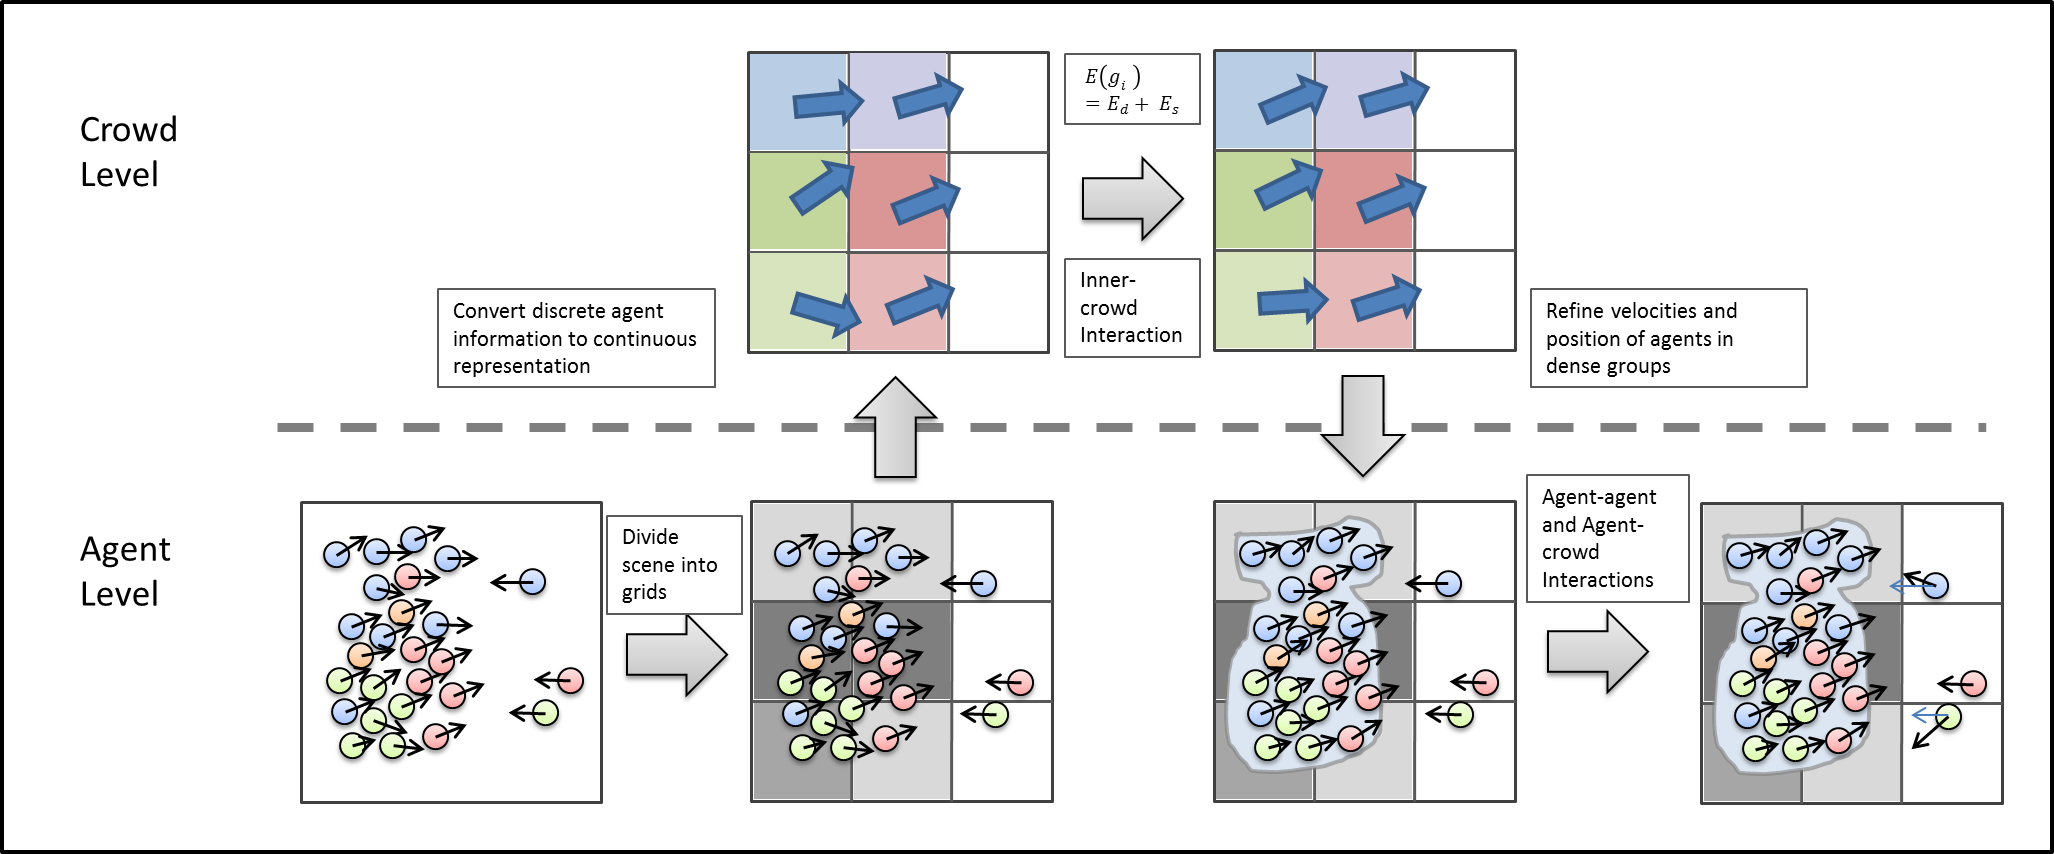
\includegraphics[width=6.4in]{images/pipeline}
  \caption{Hybrid Framework Overview. There are two levels in our framework, crowd level and agent level, represent two different views of crowd information process. The system start at agent view, assign a prefer velocity for each agent which is step 1 in section 3.3; Then the scene will be divided into several grids. Based on the location of the grids and agents inside, we converted discrete agent information into continuous representation. After that, we merged adjacent dense grids into bigger crowd. These are step 2 to 5. Then we applied Graph-Cut based algorithm for one or two iteration to smooth and optimize the velocities of adjacent dense groups which is step 6. As described in step 7, we refined velocities for each agent in dense region with the group average velocities and densities. And at the same time, we extracted the contour of dense crowds. Finally, in step 8, we add dense crowd contours as obstacles back to our agent level, and simulate agent-agent and agent-crowd interactions. In this figure, different color of agent means different personality. Different scale level means different density. When the color is darker, the density is higher. In group level, the different color of groups also represent different group traits, which will have effect on the ability of preserve the velocity of itself. However, the group traits are blind to individuals outside the crowd. Thus, when we come back to agent level, the colors of groups are replaced by gray scale density again.}
  \label{figure:pipeline}
\end{figure*}

\section{Introduction}

Crowd movement is a common but complicated and interesting phenomenon in our daily lives. Crowd simulation, user for the study of crowd behavior, has been widely applied to movies, games, and architecture, as well as in sociology and psychology research. Crowd behavior, or pedestrian behavior, is related to the behavior of each individual in the crowd. Thus, an intuitive idea is to make each agent smart, allowing it to make its own decision. This kind of method is called an agent-based method. However, agent-based methods suffer from high-dimensional computation costs, which sharply increase as the number of agent increases, limiting the scope of scenarios to which they can be applied to smaller groups of individuals. Also, some agent-based algorithms have trouble in dense crowd simulations because the high density will lead to a limited solution space, requiring more time to converge. To solve the high density and large population crowd problem, some researchers posited the idea of a continuous method, which considers people as groups, and solves the simulation problem at a macro level. Continuous methods can work well with large dense crowds, but suffer from poorer performance in low-density regions as agents may collide and overlap due to violations of the assumption of density. In order to take advantage of both methods and simulate scenarios with both sparse and dense crowd distribution, \cite{Golas:2013} proposed a hybrid solution which combines and smoothly blends agent-based methods and continuous methods.

However, in the observation of our daily life, pedestrian behavior is more than a combination of individual behavior and dense crowd movement. First, there is also interaction between the dense crowd and individuals outside the crowd. A person can choose to join or avoid a crowd encountered on the way to his target. Second, personal traits are not only individual properties but also crowd properties. As a crowd is a set of individuals with different personal traits, according to convergence theory, the behavior of the crowd is not an independent property, but based on the behavior of each individual in it \cite{Turner:1957}. There is already some research about personal traits in crowd simulation. However, they only focus on individual personality. To address the two problems and integrate them with individual behavior and dense crowd movement, we proposed our hybrid framework. In our framework, we define three types of interaction: agent-agent interaction which represents individual behavior, intra-crowd interaction which represents continuous dense crowd movement, and agent-crowd interaction which represents the decision of individuals when countering crowds. Given these three definitions, we are able to apply an appropriate interaction strategy based on the situation of the dynamic crowd movement. In addition, we integrate personal trait properties into both individuals and crowds. Thus, all three types of interactions are driven by both physical properties like position, velocity and radius, as well as personal traits.

In terms of implementation, we propose a Graph-cut based method to simulate interactions between heterogeneous dense groups within a crowd. Here, the group is a set of agents sharing the same neighborhood, which is a natural concept in continuous crowd methods. The concept of heterogeneous dense groups means that not only does each agent have personal traits, but each group also has traits added to it by its agents. So, our heterogeneous dense crowd simulation is a multi-variable optimization problem, which may have more variables than simply density and velocity. Previous work on continuous crowds are based on the assumption of homogeneous crowds, in which all agents and groups share the same personal traits. Thus, these models, such as potential field \cite{Treuille:2006} or fluid based \cite{Narain:2009}, cannot fit heterogeneous dense crowd simulation situations. To address effective heterogeneous dense crowd simulation, we consider the collisions and cooperation between adjacent groups as a multi-label optimization problem, which is to assign a label for each element in the target set and find the best overall assignment to those labels based on constraints. With this formulation, we introduce the idea of adapting intra-crowd interaction into the multi-label optimization problem, such as Graph-Cut or Belief Propagation, which has been successfully used in stereo matching, image restoration and optical flow \cite{Pedro:2004,Marshall:2003,Qingxiong:2009}, and can be applied to solve the problem of dense crowd simulation. In our work, instead of doing full iteration to achieve min-cut, we only apply a few iterations to smooth the movement of neighbor groups and reduce conflicts between groups.

Our results show that we are able to simulate the behavior of heterogeneous crowds with various agent density distributions. In our experiments, while personal traits of agents changed, we can see significant changes in crowd behavior such as aggressive dense groups \S\ref{section:6.2} and different types of agent-crowd interaction \S\ref{section:6.3}. The key contributions of our work can be summarized as follows:

\begin{itemize}
\item We propose a hybrid framework which integrates three different types of crowd behavior and personal traits.
\item We develop a graph-cut based method to simulate heterogeneous dense crowd movement.
\item We introduce agent-crowd interaction as a new type of crowd behavior and propose a method to simulate it.
\end{itemize}

\section{Related Work}

In this section, we give a brief overview of prior work on crowd simulation and multi-agent systems. There are two steps, navigation and collision avoidance, in most crowd simulation systems. Navigation, also called global-planning, is the process of finding a path from the current agent position to the goal that avoids collisions with static obstacles in the scene. There has been significant work on this topic \cite{Funge:1999,Bayanzit:2002,Lamarche:2004,Sud:2007,Sud:2008}, but we will not cover it here.
Collision avoidance is another popular area of work where a large amount of research has been done. One of the traditional ways to classify collision avoidance methods is based on the representation of crowds as either discrete or continuous. In discrete representation, also called agent-based representation, the collision avoidance decision is made by each individual agent with respect to other agents and obstacles. A number of different models like social forces \cite{Helbing:1995,Helbing:2005,Gayle:2009,Sud:2007}, sociological factors \cite{Musse:1997}, psychological factors \cite{Pelechano:2008} and synthetic-vision based steering \cite{Ondrej:2010} have been used to formulate the collision avoidance behavior of agents. There are also many methods based on the spatial and geometric relationships between agents \cite{VDBerg:2008,VDBerg:2009,Guy:2009,VDBerg:2011}. As geometrically-based methods have shown very good quality and became very popular in recent years, many other models were adapted into these methods for further quality improvement and more complicated agent behavior simulation. \cite{Guy:2010} proposed a least-effort energy model to minimize individual collision avoidance cost from an energy-optimization view. \cite{Guy:2011} introduced a personal traits model and the transformation between simulation parameters and personal-traits model based on a video user study. \cite{Kim:2012} incorporated a stress model into crowd simulation system to simulate crowd behavior during an event. \cite{Best:2014} proposed a density-filter based method to detect neighborhood density for each agent and applied a local planner to achieve better performance in various density scenarios. 

For continuous representations, agents are influenced by their dense neighborhood and have less freedom to make independent collision-avoidance decisions. Continuum theory for pedestrians flow was first proposed by \cite{Hughes:2003} and extended by \cite{Treuille:2006}. The approach of \cite{Treuille:2006} combined global planning and local collision avoidance into a single pipeline and provided good performance for medium-sized crowds with a common goal. However, this approach is not suitable for tightly packed crowds and/or varying goals. The state-of-art work of continuous methods is \cite{Narain:2009}, which combined a Lagrangian representation of individuals with a coarser Eulerian crowd model to capture discrete motions of individual agents and macroscopic flow of crowds. The work of \cite{Narain:2009} can simulate large numbers of agents at interactive rates and has good performance on dense crowds. 

To make good use of advantages of both methods, and to avoid the drawbacks, a hybridization of those two methods could be a good solution. \cite{Golas:2013} presented a long-range collision avoidance model which smoothly blends agent-based and continuous algorithms to simulate the movement of crowds with various densities. 

Besides crowd locomotion, there is also significant research on the influence of properties like personality and stress on the crowd. \cite{Durupinar:2008} proposed a method to map parameters of the HiDAC model to each agent using the OCEAN personality model to personality traits. \cite{Salvit:2011} explored the Myers-Briggs Type Indicator (MBTI) to define agent personality and ran experiments on how agents interact with the environment based on the MBTI model. \cite{Farhangian:2011} modeled recruiters’ personalities and found these can have a significant effect on team formation in organizations with temporary projects. \cite{Prada:2009} presented a FFM personality model which generates diversity interaction in the behavior of social agents in teamwork. 
Our approach focuses on more complicated pedestrian behavior in heterogeneous crowds in which both the density and personality vary from position to position, and agent to agent. To achieve this goal, we propose our hybrid framework to integrate three types of interactions between agents and crowds which are driven by both physical simulation parameters (e.g., preferred speed, radius and planning time horizon), personal traits of agents, and small agent groups in crowds \S\ref{section:3}. In \S\ref{section:4}, we introduce our continuous algorithm to address the heterogeneous dense crowd simulation problem, defined as intra-crowd interaction in our framework. The details of agent-crowd interaction about agents’ choices of avoiding or joining a crowd in their way are described in \S\ref{section:5}. We demonstrate the advantages and efficiency of our hybrid framework in \S\ref{section:6}. Finally, we conclude with the contributions and limitations of our work, and discuss the future work in \S\ref{section:7}.

\section{Hybrid Framework}
\label{section:3}
In this section, we introduce the agent model, crowd model. and the overall pipeline of our hybrid framework. There are three types of entities in our framework: agent, group and crowd. An \emph{agent} represents a single person in the system with simulation parameters and personal traits. A \emph{group} is a set of people sharing the same neighborhood. The neighborhood is defined as a 2D grid in the scene. A \emph{crowd} is a set of groups which are adjacent to other groups in the same crowd. If we consider the groups in the scene as vertices, and the adjacent relationship as edges, a crowd is a connected component of the scene. Both groups and crowds have average density, speed, and personal traits. A crowd also has a contour to support agent-crowd interaction.
\subsection{Agent Modeling}
\label{section:3.1}
We follow the definition of personal trait proposed by \cite{Guy:2010}, in which they applied the Eysenck 3-factor model \cite{Eysenck:1985} to agents. Besides personal traits, each agent also has basic simulation attributes derived from RVO  \cite{VDBerg:2009}, including, maximum neighbors’ distance, maximum number of neighbors, planning horizon, agent radius, and preferred speed. Based on linear regression in their user study, Guy et. al. provide a mapping matrix for transforming simulation parameters into personal traits. They also applied PCA to simplify the three factors into two, called PC1 and PC2, which are extroversion and carefulness. In our approach, we take simplified PC1 and PC2 traits as personal trait examples to simulate agent-agent interaction. We directly use the linear mapping matrix from \cite{Guy:2010} to transform basic simulation attributes to personal traits. After we get PC1 and PC2, we scale them to a new domain  [-1,1] to simplify later computations.
\begin{equation}
\label{eq:1}
	\binom{PC1}{PC2}= \bigl(
	\begin{smallmatrix}
	0.0 & -0.04 & 0.04 &0.75 & 0.66\\ 
	0.14 & 0.5 & 0.8 & 0.15 & -0.19
	\end{smallmatrix}\bigr)
	\begin{pmatrix}
	\frac{(Neighbor Dist.-15)}{13.5}\\ 
	\frac{(Max.Neighbors-10)}{49.5}\\ 
	\frac{(Planning Horiz.-30)}{14.5}\\ 
	\frac{(Radius-0.8)}{0.85}\\ 
	\frac{(Pref. Speed-1.4)}{0.5}
	\end{pmatrix}
\end{equation}

\subsection{Crowd Modeling}
\label{section:3.2}
Based on the method described in \cite{Narain:2009}. we define our crowd model with density, average velocity, and group personal traits to convert discrete agent information to continuous crowd information. Like \cite{Narain:2009}, we first use a Navigation Mesh as our global planning algorithm for each agent. Then the information of discrete agents is transferred to 2D grid-cells with the same size. Agents in a cell will be considered as a group. The density $\rho$ and velocity $\bar{\textbf{v}}$ can be computed as,
\begin{equation}
\label{eq:2}
 \rho = \sum_{i} \omega_\textbf{p}(\textbf{x}_i)m_i
\end{equation}
\begin{equation}
\label{eq:3}
 \bar{\textbf{v}} = \frac{\sum_{i} \omega_\textbf{p}(\textbf{x}_i)\tilde{\textbf{v}}_i}{\sum_{i} \omega_\textbf{p}(\textbf{x}_i)}
\end{equation} 

where $\textbf{x}_i$ is the position of the agent, $\tilde{\textbf{v}}_i$ is the prefered velocity of the agent, $m_i$ is the mass of each agent which are unity. 

While simulation parameters are converted into continuous representations, we can compute the group traits based on each agent’s personal traits at the same time. 
\begin{equation}
\label{eq:4}
 \bar{PC1}(\textbf{x}) = \frac{\sum_{i} \omega_\textbf{p}(\textbf{x}_i)PC1_i}{\sum_{i} \omega_\textbf{p}(\textbf{x}_i)}
\end{equation} 
\begin{equation}
\label{eq:5}
 \bar{PC2}(\textbf{x}) = \frac{\sum_{i} \omega_\textbf{p}(\textbf{x}_i)PC2_i}{\sum_{i} \omega_\textbf{p}(\textbf{x}_i)}
\end{equation} 

In this paper, we use unified weight $\omega_\textbf{p}(\textbf{x}_i)$ for all the agents in the group.

Once the cells are converted to a continuous representation, we can apply either continuous crowd or agent-based algorithms to them based on the density $\rho$ of each cell. For the $i$th cell, if $\rho_i(\textbf{x})<\rho_{min}$, it should be marked as a sparse cell and the agent-based algorithm described in \S\ref{section:5} is applied. Otherwise, it should be marked as a dense cell, and we refine the crowd information by minimizing the inter-group collision energy described in (\S\ref{section:4.1} and \S\ref{section:4.2}). Then, the density $\rho_i(\textbf{x})$ and velocity $v_i(\textbf{x})$ at the agent position can be interpolated from cell density and cell velocity using the bilinear interpolation mentioned in \cite{Treuille:2006}. We can get the final velocity of each agent by interpolating between the continuum velocity $v_i(\textbf{x})$ and the agent's preferred velocity $\tilde{\textbf{v}}_i$, depending on the crowd density $\rho_i(\textbf{x})$ at its location:

\begin{equation}
\label{eq:6}
\textbf{v}_i = \tilde{\textbf{v}}_i + \frac{\rho(\textbf{x}_i)}{\rho_{max}}(\textbf{v}(\textbf{x}_i) - \tilde{\textbf{v}}_i)
\end{equation}

\subsection{Overview of the Pipeline}
\label{section:3.3}
The computation pipeline of our hybrid framework can be summarized as follows:
\begin{enumerate}
\item Compute a preferred velocity $\tilde{\textbf{v}}_i$ for each agent using the Navigation Mesh.
\item Divide our scene into uniform-sized 2D grid-cells from the top view.
\item Compute the density $\rho$, velocity $\bar{\textbf{v}}$ and personal traits for each 2D cell
\item Mark grids as either dense or sparse based on the density $\rho$ of each cell (see \S\ ref{section:3.2})
\item Merge adjacent dense cells as crowds (see \S\ref{section:5.1})
\item Reduce inter-group collisions and refine group velocities using a graph-cut based method (see \S\ref{section:4}) for agents in high density cells.
\item Update velocities of agents in dense regions by group velocities (see \S\ref{section:3.2}) and extract contours and average velocities for dense groups (see \S\ref{section:5.1}).
\item Add dense group contours to agent-based algorithm as moving obstacles and simulate agent-agent and agent-crowd interactions (see \S\ref{section:5.2}).
\end{enumerate}

\begin{figure}
  \centering
  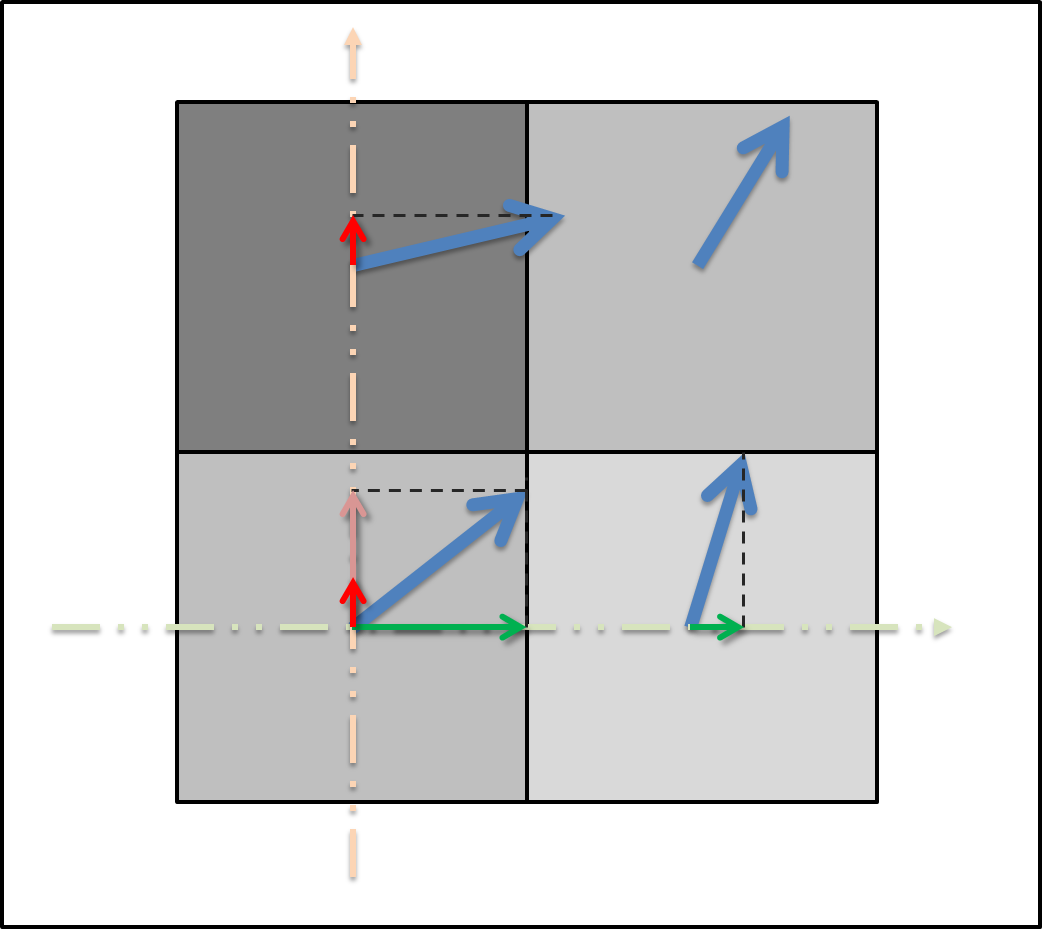
\includegraphics[width=2.0in]{images/graph_cut_model}
  \caption{Illustration of Label Definition in Graph-Cut Based Continuous Model. In this figure, the gray scales represent density like Figure 1. The left-top grid is the darkest grid and has maximum density while the other three are not full. We illustrated the labelling process for the left-bottom grid. In the left-bottom grid, the light red axis is the vertical axis, while the light green axis is the horizontal axis. From the figure, we can see that as we are using a 4-neighbor system, the only “pressure” from the top or bottom grid is on vertical axis. And the forces from the left and right grids only push the horizontal boundaries of current grid. Thus we separate horizontal and vertical into two independent processes to have more labels on both axis and achieve better precision. The blue arrows are the average velocities of girds. The red arrows are the vertical projection of velocities while the green arrows are horizontal projections. As the left-top grid reaches its maximum density, we cannot put more agents into it. Thus the vertical velocity of the left-bottom grid should be smaller than its vertical velocity. So, the originally vertical velocity (pink arrow) is no longer available and the label larger than the value will be assigned a very high penalty value during the Graph-Cut process.}
  \label{figure:graphcutmodel}
\end{figure}

\section{Intra-Crowd Interaction}
\label{section:4}
According to our observations of dense crowd behavior, collisions, merging, and negotiations constantly happen between groups in dense crowds. However, unlike local collision avoidance strategies for agents which can be considered as rigid bodies, groups are highly influenced by neighbor groups and have the tendency to share the same movement. We also find that groups have traits which are determined by the personal traits of the people inside them. However, previous work like \cite{Treuille:2006} and \cite{Narain:2009} are based on the assumption of homogeneous groups. Inspired by our observations and aiming to simulate interactions between groups with different traits, we propose a minimal energy model to describe and solve intra-crowd interaction for heterogeneous groups.


\subsection{Energy Modeling}
\label{section:4.1}
We define intra-crowd interaction as a labeling problem by assigning to each cell $g_i$ a label $l_i$. Each cell is a group of agents. As the influences from horizontal and vertical directions are independent (from different neighbor groups) in one simulation step, we call the energy minimization process twice to minimize collision energy of the horizontal and vertical directions separately. Thus, for each optimization pass, we could have $m$ labels by dividing horizontal or vertical space into m pieces. Each of the labels represents the scale of velocity on the $x$ or $y$ axis. We assign at least 81 labels for each direction to approximate the discrete velocity we got from Graph-Cut to the optimal value. The energy function $E$, composed of a data energy $E_d$ and a smoothness energy $E_s$, is defined as:

\begin{equation}
\label{eq:7}
E(g_i) = E_d + E_s
\end{equation}

The data energy $E_{d}(g_i)$ is the sum of data cost of each cell with a label $d(l_i)$. In our energy model, the data cost $d_{i}(l_i)$ is defined as the product of a scale value $\pi_i$ and the absolute distance between the horizontal or vertical projection of the average cell velocity $\bar{\textbf{v}}(g_i)$ and the value of the selected label $v(l_i)$. Data cost represents the effort of the group to change its velocity on $x$ or $y$ axis to certain label.

\begin{equation}
\label{eq:8}
E_{d}(g_i) = \sum_{i}\pi_i*d_i(l_i) = \sum_{i}\pi_i*|\bar{\textbf{v}_x}(g_i) - v(l_i)|
\end{equation}

\begin{equation}
\label{eq:9}
\pi_i = f(\sigma ) = \alpha\bar{{PC1}_i} + \beta\bar{{PC2}_i}
\end{equation}

The scale value $\pi_i$ is computed by the group traits $\bar{{PC1}_i}$ and $\bar{{PC2}_i}$. Although there are several potential functions $f(\sigma)$ to compute the scaled weight $\pi_i$ with different personal traits model $\sigma$,
in this paper, we choose a simple linear equation of two traits to give an estimated value of $\pi_i$. A more precise formulation will be given in future work with measurement data. In our experiment, the $\alpha$ and $\beta$ will be set as 0.3 and -0.3, respectively

The smoothness energy $E_s(g_i)$ represents the velocity difference between neighboring grids. We use a standard 4-neighbor system for dense grids, so that the smoothness energy is the sum of spatially varying horizontal and vertical neighbor smoothness costs $V_ij(l_i,l_j)$, where if $i=(p,q)$ and $j=(s,t)$ then $|p-s| + |q-t| = 1$. Letting $N$ denote the set of all such neighboring cell pairs, the smoothness energy is
\begin{equation}
\label{eq:10}
E_s = \sum\limits_{\left\{ {i,j} \right\} \in \mathcal{N}} V(\left|l_i,l_j\right|)
\end{equation}

In equation \ref{eq:10}, $V(\left|l_i,l_j\right|)$, also can be written as $V(\Delta l)$, is a non-decreasing function of the label difference, and can be directly computed as the absolute difference between two labels. $V(\left|l_i,l_j\right|)$ is adjusted to restrict the maximum density of each group (see \S\ref{section:4.2}).

\subsection{Constraints}
\label{section:4.2}
While trying to reach the minimal energy cost for inter-group collisions, we should also keep the density of each group below the maximum density $\rho_{max}$ because of the incompressibility of the human body. If the density of cell $g_i$ is below $\rho_{max}$, agents can be pushed into the cell from neighboring cells. Otherwise the cell is incompressible. The smooth term should be,

\begin{equation}
\label{eq:11}
V(\left|l_i,l_j\right|) = \left\{ 
{\begin{array}
{*{20}{c}}
{\left| {{l_i} - {l_j}} \right|,  {\rho _i} \le {\rho _{max}}}\\
{\Delta _{max},  {\rho _i} > {\rho _{max}}}
\end{array}} 
\right.
\end{equation}
where $\Delta_{max}$ is a constant value as a penalty of labels which could lead to potentially overcrowded.

\subsection{Obstacles and Rearrangement}
\label{section:4.3}
If there are obstacles in the scene, we use a similar strategy as \cite{Narain:2009}. For each cell, we compute the fraction $f$ of area that is inside the navigation mesh, and multiply the $\rho_{max}$ by the fraction $f$ as the new maximum density for this cell. 
After each continuous crowd algorithm step, we rearrange overlapped agents to solve inter-agent collisions which often happen in continuous crowd algorithms. We divide the cell into several bands along the average velocity direction, and give agents a band ID. Then, we traverse each band to check if there are agents the collide with other agents in the next band. If they overlap, we move the agent in the next band slightly in another direction until they are no longer overlapped. We also push overlapped agents from the middle of each band to both sides in case two agents in the same band are overlapped. For each simulation frame, we do 10 iterations of rearrangement to achieve smooth movement for every rearranged agent.

\section{Agent-Crowd Interaction}
\label{section:5}
After crowd behavior, we introduce individual behavior including agent-agent interaction and agent-crowd interaction. For agent-agent interaction, we simply apply the RVO algorithm to achieve good quality of collision avoidance behavior between agents. In this section, we mainly focus on agent-crowd interaction. Agent-crowd interaction simulation is based on the personal traits of individual agents in low density regions, and spatial information of both those agents and the crowds nearby. Thus, we first extract the contour of crowds as the boundary of a moving obstacle from an agent’s point of view. Then, the decision of whether avoid or join the crowd is determined by the personal traits of the agent. These algorithms are described in detail in \S\ref{section:5.1} and \S\ref{section:5.2}.

\subsection{Dense Crowd Contour Extraction}
\label{section:5.1}
After we convert discrete agent information into continuous representation, and mark each group as dense or sparse by its density, we merge adjacent groups into crowds. By considering the groups as vertices, and connections between groups as edges, we can construct a graph structure to represent the relationship between groups. Then we can simply apply a connected-component labeling algorithm to extract crowds from the graph. During the process, we can also record neighbors of each grid, which will be useful during building neighbor links for smoothing terms.

In the next step, we extract the contour $C_i$ of each crowd $c_i$. As we only need rough contours to be moving obstacles in agent-crowd interactions, we use the simple contour extraction algorithm described below,

\begin{itemize}
\item For each group $\mathcal{G}_i$ DO
\begin{enumerate}
\item group $g_j$ in the crowd by its vertical center position in ascending order, positions of group centers on the top and bottom of the list are marked as $p_{min}$ and $p_{max}$
\item For groups in the same vertical level, sort again by horizontal position in ascending order, and mark the position of group center on the top and bottom of the list as $p_{j, left}$ and $p_{j, right}$.
\item Connect points in such an order: $p_{min}$, $p_{1, left}$, $p_{2, left}$, $\cdots$, $p_{N-1, left}$, $p_{N, left}$, $p_{max}$, $p_{N, right}$, $p_{N-1, right}$, $\cdots$, $p_{2, right}$, $p_{1, right}$ and $p_{min}$ to create a contour polygon $C_i$. Here, $N$ is the number of different vertical values of all the groups.
\end{enumerate}
\item END for loop
\end{itemize}

\subsection{Avoid or Join, Agent Behaviors}
\label{section:5.2}
To simulate avoid or join behaviors, we convert the PC1 and PC2 traits to the minimum distance to crowds and maximum tolerable density, respectively. We began with some observations about individual pedestrian behavior when encountered with crowds on the path. Based on those observations, we came up with two empirical conclusions. With a higher PC1, which means more extroverted, an agent is more likely to walk directly into a crowd in its way on the way to the target. Thus, the minimum distance to crowds should be smaller. Otherwise, the agent would choose to avoid the crowds earlier. An agent with a higher PC2, which means he has a careful personality, will try to avoid walking into a very dense crowd to protect himself. So an agent with a higher PC2 will have a lower maximum tolerable density. The ranges of each parameter are shown in table \ref{table:1}

\begin{table}  
\centering  
\begin{tabular}{|c|c|c|c|}
\hline 
Parameters & Min & Max & Equation \\ 
\hline 
PC1 & -1 & 1 & - \\ 
\hline 
PC2 & -1 & 1 & - \\ 
\hline 
Min. Dist. & 0 & $d_{min}$ & $d_{min}*\frac{(1 - PC1)}{2}$ \\ 
\hline 
Max. Density & 0 & $\rho_{max}$ & $\rho_{max}*\frac{(1 - PC2)}{2}$ \\ 
\hline 
\end{tabular} 
\caption{Range of agent-group simulation parameters}  
\label{table:1}
\end{table}

Then, for a crowd with average density $\rho$ and velocity $\textbf{v}_c$, and an agent with velocity $\textbf{v}_a$, if $\rho \geq Max. Density$, then we set the planning horizon for obstacles as $\frac{Min.Dist.}{\sqrt{(\textbf{v}_a-\textbf{v}_c)^2}}$, which is the time for the agent to avoid the crowd. Otherwise, The crowd will not be treated as an obstacle to this agent.

Based on our experience, crowds rarely change their speed and direction for several individuals while agents are not close enough to the crowds. When individuals get close enough, they will be absorbed into the crowd automatically due to the method we described in \S\ref{section:3.2}. Thus, behaviors like an agent walking through a crowd will be part of the continuous crowd algorithm instead of agent-crowd interaction.
\begin{figure}
  \centering
  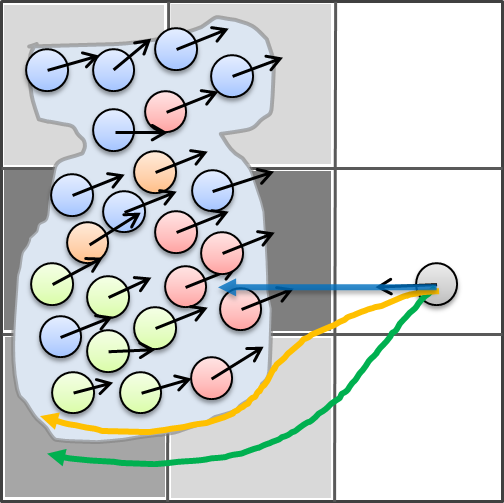
\includegraphics[width=1.2in]{images/agent_crowd_choices}
  \caption{Illustration of Different Choices for Agents with Different Personalities. In this figure, an agent in gray is an individual encounter with a dense crowd. The gray color represent an arbitrary personality. There are three types of choices in three colors, blue, orange and green. The green trajectory represents a low extraversion and high carefulness personality which leads to early avoidance behavior. The orange one represents a personality that both extraversion and carefulness are high. The more extraversion a person is, the later he would choose to avoid the dense crowd. Thus the trajectory has a big curve when it is close to the crowd. The blue one represents a low carefulness personality. A careless agent will just walk through the dense crowd. And the less carefulness it is, the higher density it could tolerate.}
  \label{figure:agentcrowdchoice}
\end{figure}

\section{Result}
\label{section:6}
\subsection{Performance}
\label{section:6.1}
Our approach is implemented in C/C++. We provide our run-time performance on an Intel Core i7 at 2.9GHz with four cases in Table \ref{table:2}. We measure the per-frame performance of both the agent-based module and the continuous module, and the entire hybrid pipeline. From Table \ref{table:2}, we can see that the agent-based portion is the performance bottleneck when there are large numbers of agents in the scene. A pure continuous algorithm, in our case the Graph-Cut based method, shows much better performance when the number of agents increases to 10k. When the agent number is around 5k, our method could reach real-time performance for most cases. Although the performance is not very impressive, it was still close to other hybrid solutions (please refer to Table 1 in {Golas:2013}) while we provided more complicated agent and crowd behaviors. And we can achieve better performance by taking less iterations of Graph-Cut and rearrangement, or decrease the density threshold to make more grids to be applied continuous algorithm.

\begin{table}  
\centering  
\begin{tabular}{|c|c|c|c|}
\hline 
Scene & \# Agent & Modules & Time(ms) \\ 
\hline 
Crossing & 500 & Agent-based & 0.7 \textasciitilde 3.8 \\ 
 &  & Continuous & 0.2 \textasciitilde 2.7 \\ 
 &  & Total Hybrid & 1.1 \textasciitilde 6.9 \\ 
\hline 
4 Groups & 4000 & Agent-based & 6.6 \textasciitilde 22.1 \\ 
 &  & Continuous & 24.2 \textasciitilde 42.5 \\ 
 &  & Total Hybrid & 37.4 \textasciitilde 49.0 \\ 
\hline 
4 Groups L & 10000 & Agent-based & 60.7 \textasciitilde 373.4 \\ 
 &  & Continuous & 36.6 \textasciitilde 61.5 \\ 
 &  & Total Hybrid & 107.3 \textasciitilde 379.5 \\ 
\hline 
4 Groups XL & 25000 & Agent-based & 0.7 \textasciitilde 436.1 \\ 
 &  & Continuous & 25.7 \textasciitilde 170 \\  
 &  & Total Hybrid & 143.7 \textasciitilde 480.3 \\ 
\hline 
\end{tabular} 
\caption{Performance of our methods in four scenes. We give both minimum time and maximum time here. There are significant differences between min and max time because that the agent could either be applied discrete or continuous algorithms. Thus the time cost is not very stable during frames. In all scenes, the map is divided into cells sized 20 units. One unit is close to the diameter of an agent.}  
\label{table:2}
\end{table}

\subsection{Heterogeneous dense crowd experiment}
\label{section:6.2}
We compare different crowd behaviors in heterogeneous and homogeneous crowds. In our experiment, shown in \ref{figure:heterogeneouscrowd}, we define two groups: the experiment group and the control group. In the experiment group, there are two groups of agents with different personal traits. Thus the group traits were different. Red agents were set to be more aggressive, meaning higher extroverted and lower carefulness values. Green agents were relatively more shy and assigned lower extroverted and higher carefulness personal traits. So the red group was relatively more aggressive than the green group. In the control group, all the agents in red and green share the same personal traits. In Figure X, the left side is the experiment group while the right side is the control group. From top to bottom, the first row is the original position of the two groups, which is the same for both experiment and control groups. The second row is a later frame. In the experiment group, some of agents from the red group “invade” into green group while few green agents venture into the red group. In the control group, both groups are exchanging agents along the middle line. The third row is even later, and in the experiment group, the red group is obviously in a dominant position. In the control group, there are no noticeable signs showing which group is more dominant.

\subsection{Agent-Crowd Interaction Experiment}
\label{section:6.3}
In this experiment, we compare the different behaviors when agents with different personal traits encounter a dense crowd. There are three different choices in such situations according to the strategy introduced in \S\ref{section:5.2}. The first choice is to avoid the crowd from a distant place. Agents with lower extroversion (PC1) and higher carefulness (PC2) will have the first choice as higher carefulness leads to a behavior of avoiding dense crowds and not getting hurt, and lower extroversion leads to keeping a greater distance from dense crowds. The second choice is based on both high PC1 and PC2, which leads to avoiding the crowd when the crowd is rather close. The third choice happens when PC2 is high, which means the agent is too careless to pay attention to the potential damage of being in a dense crowd. In this case, the agent will choose to join the crowd. The choice here is also related to the density, distance, and velocity of the crowd. In the experiment, shown in Figure X, the left group is individual agents (red) with lower extroversion and higher carefulness that encounter a dense crowd (green). From the position and trajectories of the agents, we can see that those agents have perfectly bypassed the dense crowd. In the middle group, agents have both high extroversion and carefulness. Thus, one of the agents (the second one from left) is not able to avoid the crowd, while others just turn a little to get avoid the crowd. In the right group, the careless agents just go through the crowd. From this experiment, we can see that different choices are made based on the personality of each agent and the environment (dense crowds). 


\begin{figure*}
  \centering
  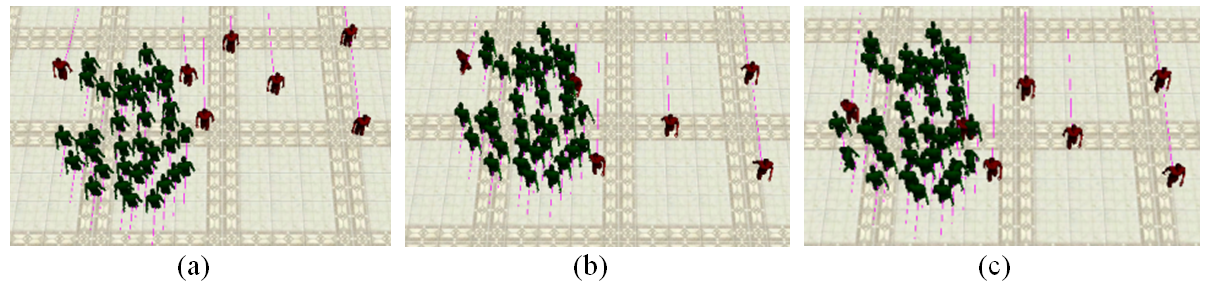
\includegraphics[width=6.4in]{images/agent_crowd}
  \caption{Different Choices When Encountering A Crowd. (a) represents the behavior of individual agents with low extroversion and high carefulness. (b) represents the behavior of individual agents with both high extroversion and carefulness. (c) represents the behavior of individual agents with lower carefulness. Compare the three pictures from (a) to (c). In (a), all the agents successfully bypass the dense crowd. In (b) the three agents in the left are trying to avoid the dense crowd, however, the second left agent fails to do so as he is already too close to the crowd, and so becomes part of it. In (c), as agents are careless, they just walk through the crowd. Noticeable differences between each choice could be found by looking at the trajectory and orientation of each red agent, which reveals that the choices are affected by personalities.}
  \label{figure:agentcrowd}
\end{figure*}

\section{Conclusion and Future Work}
\label{section:7}
In this paper, we present a hybrid framework for heterogeneous crowds with various densities. We define three types of interactions in crowd behaviors, agent-agent interaction, agent-crowd interaction and intra-crowd interaction. Our hybrid framework enables the simulation of more realistic crowd movement with combinations of the three interactions, especially the agent-crowd interaction, which is first introduced in crowd simulation. We formulate and develop our Graph-Cut based model to reduce collision energy between heterogeneous dense groups housing agents with different personal traits inside. 
There are some limitations in our approach. First, because the formulation of the energy model is based on a Graph-Cut algorithm, we are using discrete values to represent a continuous interval. We are looking for interpolation methods to provide continuous values for the energy model. Secondly, our pipeline is not implemented in parallel, which limits our performance. A GPU-based implementation is needed, and is planned as future work. We are also looking for accurate pedestrian locomotion measurements to support and modify our agent and group model.

\begin{figure}
  \centering
  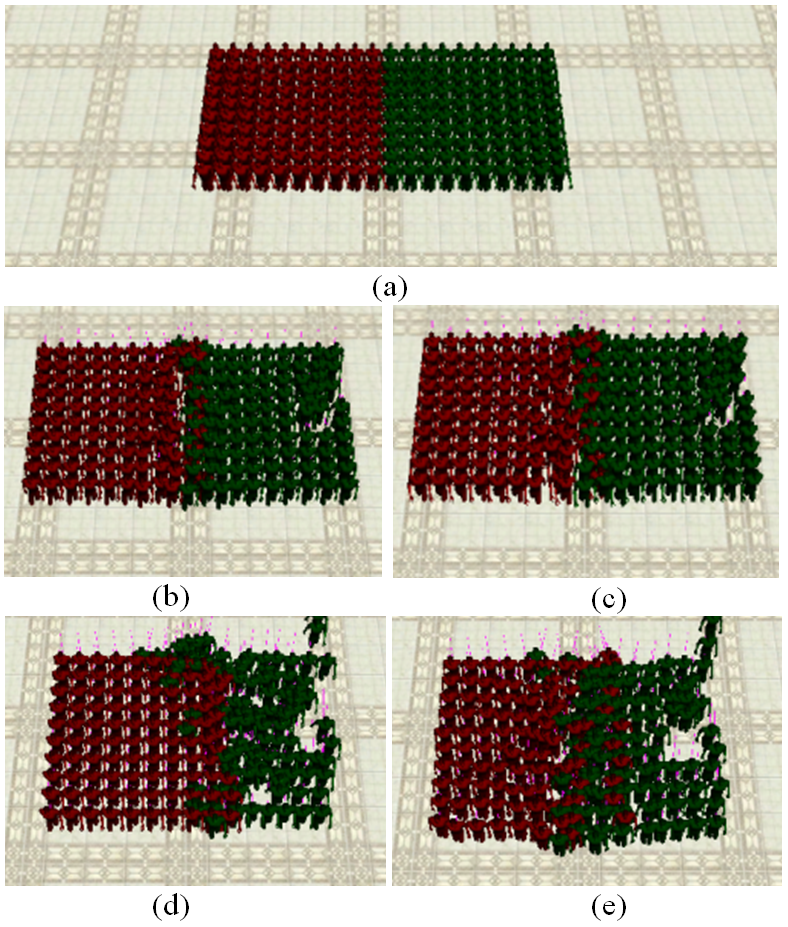
\includegraphics[width=2.8in]{images/heterogeneous_crowd}
  \caption{Heterogeneous Dense Crowd vs. Homogeneous Dense Crowd. (a) is the original position for both crowds. (b) and (d) are later frames of the heterogeneous dense crowd. (c) and (e) are later frames of the homogeneous dense crowd. In the hetereogeneous dense crowd, the red group is relatively more aggressive while all groups are the same in homogeneous dense crowd. The two groups are assigned intersecting paths, which means they must encounter and compete with each other during the simulation. Comparing the left column (heterogeneous) to the right column (homogeneous), we can see siginificant differences in that the aggressive group (red in the left column) shows its dominance in this compitition between the two groups.}
  \label{figure:heterogeneouscrowd}
\end{figure}

\bibliographystyle{acmsiggraph}
\bibliography{reference}
\end{document}


